\section{Data preparation}

Once the dataset is captured and stored, the data still has to be formatted and prepared to be fed to our models. We decided to alter the recordings as little as possible, since it is very valuable to have raw data in projects like this one. This means any modification of the data is done at runtime. This section describes the formatting and preprocessing applied to the datasets.

\subsection{Environment}

We used python to work with our datasets and to write the models described in next section. Visualizations were done in \texttt{Jupyter notebooks} using \texttt{matplotlib}. Data processing was achieved in a python project using \texttt{numpy} to read and manipulate the data and \texttt{scipy}'s signal processing library.

% -------------------------------------------------------------------------------------------------------------
\subsection{Data partitioning}

\subsubsection{Raw partitioning}

Our first approach with the datasets was to segment each recording in windows of size $n$. Inspired by \textcite{youssef_machine_2017}, we made the window size a parameter, so that we could tune it.

The result for each tag is an array of windows, each comprised of $n$ complex samples. If the number of samples in a tag's recordings is of size $L$, then this array contains $L/n$ windows.

\subsubsection{Detecting communications}

It was soon clear that feeding the raw data without at least selecting segments that actually contained communications would not yield fantastic results. Indeed, most windows would contain only the carrier signal generated by the reader. These long segments of the signal contain little to no meaningful information. This is why we used peak detection algorithms to detect actual communications and filter out the uninteresting parts of the signal.

\begin{figure}[htbp!]
  \centering
  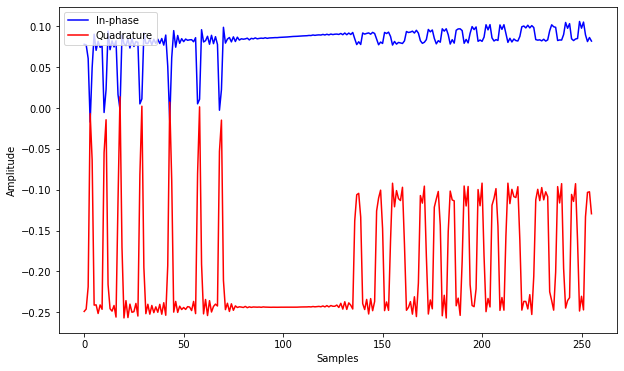
\includegraphics[scale=0.55]{figures/dataprep_window.png}
  \caption{Visual example of a window of size $n = 256$}
  \label{fig:window}
\end{figure}

\textbf{Do we use height or prominence?} An example of a resulting window can be seen in figure \ref{fig:window}.

\subsection{Input formatting}

Once our data is filtered and partitioned for input, the question of the format comes up. Indeed, a machine learning model will not accept complex numbers as input without adapting the loss function. This can be done without great difficulty, but most of the research we considered preferred representing the data as a two-dimensional array comprised of two float arrays: one for the real parts and the other for the imaginary parts. Figure \ref{fig:2din} shows a representation of the input after the windows were created and formatted this way.

\begin{figure}[htbp!]
  \centering
  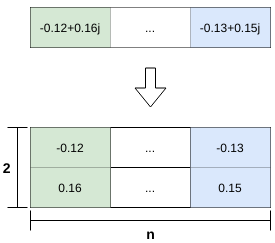
\includegraphics[scale=0.75]{figures/dataprep_2d.png}
  \caption{Format for the two-dimensional input}
  \label{fig:2din}
\end{figure}

For our experiments with SVMs, such a representation wasn't appropriate since SVMs don't accept multidimensional inputs. This is why we propose two formatting options: "2D" for the neural networks and "1D" for the SVM. The latter appends the array containing the imaginary parts to the array containing the real parts, as shown in figure \ref{fig:1din}.

\begin{figure}[htbp!]
  \centering
  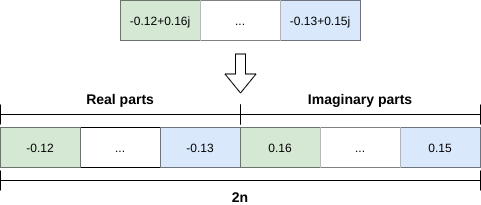
\includegraphics[scale=0.75]{figures/dataprep_1d.png}
  \caption{Format for the simple input}
  \label{fig:1din}
\end{figure}

% -------------------------------------------------------------------------------------------------------------
\subsection{Preprocessing}

normalization (amplitude, detrending?)

CWT
